\section{Methods}\label{methods}

Fully dense neural network (NN) architectures, such as the one shown in Figure~\ref{fig:nn-1}, perform a sequence of affine transformations, ${\bold z}_i \leftarrow \boldsymbol\theta_i {\bold x}^{(i)}$, followed by element-wise functional operations, $\sigma({\bold z}_i)$ to introduce non-linearity at each layer; that is, each layer stretches and distorts the underlying space.
\begin{figure}[htbp]
\begin{center}
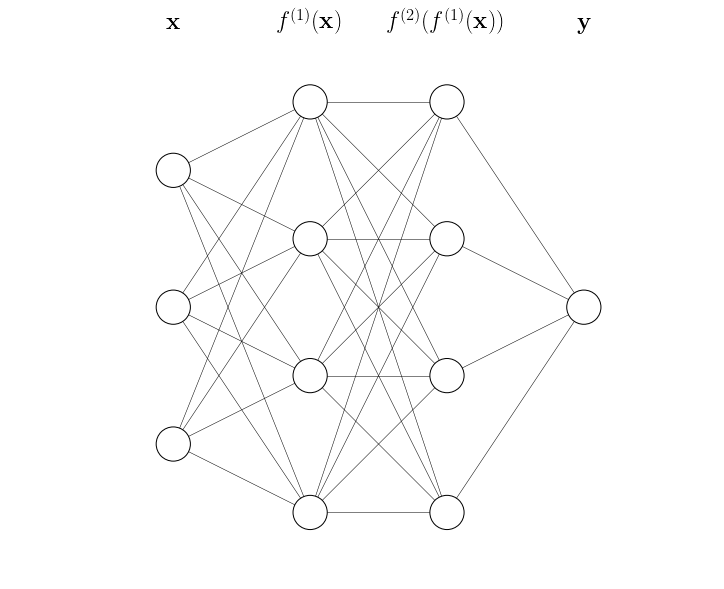
\includegraphics[width=0.8\textwidth]{fig/neural-network-01}
\caption{Schematic view of a fully dense neural network. Each sequence of affine and non-linear transformations are captured in the function, $f_i({\bold x}): {\bold x}^{(i+1)} \leftarrow \sigma(\boldsymbol\theta_i {\bold x}^{(i)})$}
\label{fig:nn-1}
\end{center}
\end{figure}

The resulting network,
\begin{equation}
	f(x) = \sigma(\boldsymbol\theta_n \sigma(\boldsymbol\theta_{n-1} \sigma(\ldots \boldsymbol\theta_2 \sigma(\boldsymbol\theta_1{\bold x}))))
	\label{eqn:nn analytical form}
\end{equation}
is an arbitrary function generator, but at present, the network weights $\boldsymbol\theta_i$ can not map back to analytic forms that capture and describe the underlying physics. There are, however, many such mappings through polynomial series expansions,
\begin{equation}
	f(x) = \sum_{n=0}^\infty a_n x^n
\end{equation}

We hypothesize that the physics of a process can be extracted by fitting the polynomial expansions of known physical relationships to the polynomial coefficients of a polynomial series expansion of Equation~(\ref{eqn:nn analytical form}).

Although ReLU (rectified linear units) have become a more common activation function, its discontinuity at $x = 0$ requires an infinite series to fully capture the behavior at this transition. However, the sigmoid function,
\begin{equation}
	\sigma(x) = \frac{1}{1 + e^{-x}}
	\label{eqn:sigmoid}
\end{equation}
is a special case of the generating function for the Euler polynomial coefficients,
\begin{equation}
	\frac{2e^{x t}}{1 + e^t} = \sum_{n=0}^\infty E_n(x) \frac{t^n}{n!}
\end{equation}
where, for $x = 0$,
\begin{equation}
	\sigma(x) = \frac{1}{2} \sum_{n=0}^\infty E_n(0) \frac{(-1)^n}{n!}.
	\label{eqn:sigmoid Euler expansion}
\end{equation}

The Euler polynomials at $x=0$,
\begin{equation}
	E_n(0) = -2(n+1)^{-1} \left( 2^{n+1} - 1 \right) B_{n+1}
\end{equation}
where $B_n$ is the $n^\textrm{th}$ Bernoulli number. Since Bernoulli numbers of odd index, with the exception of $B_1$, are zero, $E_i(0) = 0$ for $i = 2, 4, 6, \ldots, 2n$. Therefore, the summand and limits of Equation~(\ref{eqn:sigmoid Euler expansion}) change to
\begin{equation}
	\sigma(x) = \frac{1}{2} - \frac{1}{2} \sum_{n=1}^\infty \left( \frac{E_{2n-1(0)}}{(2n-1)!} \right) x^{2n-1}.
\end{equation}

The series representation of $E_{2n-1}(x)$
\begin{equation}
	E_{2n-1}(x) = \frac{(-1)^n 4 (2n - 1)!}{\pi^{2n+1}} \sum_{k=0}^\infty \frac{\cos [(2k + 1) \pi x]}{(2k + 1)^{2n}}
\end{equation}
such that,
\begin{equation}
	E_{2n-1}(0) = \frac{(-1)^n 4 (2n - 1)!}{\pi^{2n+1}} \sum_{k=0}^\infty \frac{1}{(2k + 1)^{2n}}
\end{equation}
and therefore,
\begin{eqnarray}
	\sigma(x) & = & \frac{1}{2} - 2 \sum_{n=1}^\infty \frac{(-1)^n}{\pi^{2n}} \left( \sum_{k=0}^\infty \frac{1}{(2k+1)^{2n}} \right) x^{2n-1} \\
		& = & \frac{1}{2} - 2 \sum_{n=1}^\infty \frac{(-1)^n}{\pi^{2n}} \left( 4^{-n} \left( 4^n - 1 \right) \zeta(2n) \right) x^{2n-1} \nonumber \\
		& = & \frac{1}{2} - 2 \sum_{n=1}^\infty \left( \frac{-1}{4\pi^2} \right)^n \left( 4^n - 1 \right) \zeta(2n) x^{2n-1} \nonumber \\
		& = & \frac{1}{2} - 2 \sum_{n=1}^\infty a_n x^{2n - 1},\ a_n = \left( \frac{-1}{4\pi^2} \right)^n \left( 4^n - 1 \right) \zeta(2n)
		\label{eqn:sigmoid zeta expansion}
\end{eqnarray}